\documentclass{article}
\usepackage[utf8]{inputenc}
\usepackage{graphicx}
\usepackage{amssymb}
\usepackage{physics}
\title{statemech HW 2}
\author{iwanseth }
\date{January 2020}

\begin{document}

\maketitle

\section{problem one}
\begin{flushleft}
\textbf{question: } there are six dice rolled, how many N elementary events are there?
\bigbreak
\textbf{solution: } since order matters for micro states the number of micro states is
\[ 6*6*6*6*6*6= 6^6\]
\[ \therefore N=6^6=46656\]

\section{problem two}
\textbf{question:} find the probability that each micro state is realized
\bigbreak
\textbf{solution:} each micro state has equal probability of happening, and each microstate happens only once. that means each microstate has a $\frac{1}{46656}$ chance of happening

\section{stochastic variable, problem three}
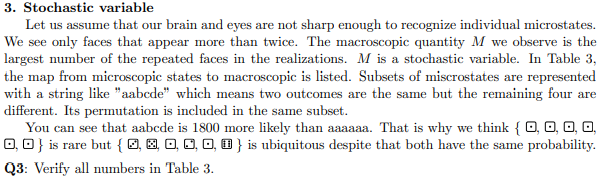
\includegraphics[scale=.7]{question3.png}
\centerline{ 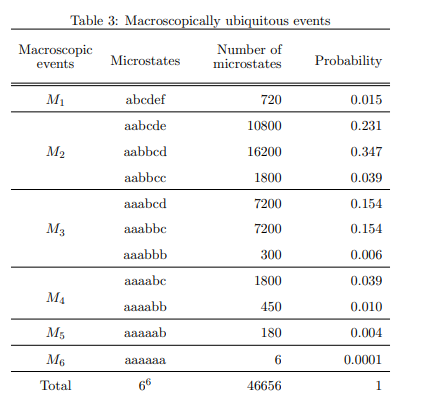
\includegraphics[scale=.8]{table3.png}}\\
\textbf{solution:}\\
for the first line in chart, $M_1$, all the numbers on the dice are different. this leads to \\
\[ 6*5*4*3*2*1=720\]
for $M_2$ there are multiple ways, therefore we will use the binomial coefficient \[ \mqty(N\\N_1)= \frac{N!}{N_1!(N-N_1)!} \]



so number of micro states for $M_2$ is

\textbf{mirostate aabcde:}
\[ 6*1*5*4*3*2*\mqty(6\\2)=\frac{6!}{1!}*\frac{6!}{2!\left(6-2\right)!}\]
\[ \rightarrow \text{Micro state} = 10800 \text{ and probability} = \frac{10800}{46656}=.2319\]

\textbf{mirostate aabbcd:}
\[ 6*1*5*1*4*3*\mqty(3\\2)\mqty(6\\2)=\frac{6!}{2!}*\frac{3!}{2!\left(3-2\right)!}\frac{6!}{2!\left(6-2\right)!}\]
the extra binomial coefficient, 3 choose 2, comes from turning aabbcd into ABC. it gives the different order that the two pair can be in
\[ \rightarrow \text{Micro state} = 16200 \text{ and probability} = \frac{16200}{46656}=.3479\]

\textbf{mirostate aabbdd:}
\[ 6*1*5*1*4*1*\mqty(3\\3)\mqty(6\\2)=\frac{6!}{3!}*\frac{3!}{3!\left(3-3\right)!}\frac{6!}{2!\left(6-2\right)!}\]

\[ \rightarrow \text{Micro state} = 1800 \text{ and probability} = \frac{1800}{46656}=.03865\]

\textbf{$M_3$}\\
\textbf{mirostate aaabcd:}
\[ 6*1*1*5*4*3*\mqty(3\\3)*\mqty(6\\3)=\frac{6!}{2!}*\frac{6!}{3!\left(6-3\right)!}\]

\[ \rightarrow \text{Micro state} = 7200 \text{ and probability} = \frac{7200}{46656}=.1546\]

\textbf{mirostate aaabbc:}
\[ 6*1*1*5*1*4*\mqty(3\\2)\mqty(6\\3)=\frac{6!}{3!}*\frac{3!}{2!\left(3-2\right)!}\frac{6!}{3!\left(6-3\right)!}\]

\[ \rightarrow \text{Micro state} = 7200 \text{ and probability} = \frac{7200}{46656}=.1546\]
\textbf{microstate aaabbb:}\\

\[ \frac{6!}{4!}*\frac{6!}{3!\left(6-3\right)!}= 600\]
but we have duplicate state cause the permutation with a=1 and b=6 are repeated when b=1 and a=6. so we divide by 2
\[ \Rightarrow microw state = 300 \text{and probability }= 300/46656=.006\]

\textbf{$M_4$}\\
\textbf{microstate aaaabc:}
\[ 6*1*1*1*5*4*\mqty(6\\4)=\frac{6!}{3!}*\frac{6!}{4!\left(6-4\right)!}\]
\[ \rightarrow \text{Micro state} = 1800 \text{ and probability} = \frac{1800}{46656}=.039\]

\textbf{microstate aaaabb:}
\[ 6*1*1*1*5*1*\mqty(6\\4)=\frac{6!}{4!}*\frac{6!}{4!\left(6-4\right)!}\]
\[ \rightarrow \text{Micro state} = 450 \text{ and probability} = \frac{450}{46656}=.01\]

\textbf{$M_5$}\\
\textbf{aaaaab}
\[ 6*1*1*1*1*5*\mqty(6\\5)=\frac{6!}{4!}*\frac{6!}{5!\left(6-5\right)!}\]
\[ \rightarrow \text{Micro state} = 180 \text{ and probability} = \frac{180}{46656}=.004\]
\textbf{$M_6$}\\
\textbf{aaaaaa}
\[ 6*1*1*1*1*1*\mqty(6\\5)=\frac{6!}{5!}*\frac{6!}{6!\left(6-6\right)!}\]
\[ \rightarrow \text{Micro state} = 6 \text{ and probability} = \frac{6}{46656}=.0001\]

\section{Question4}
\textbf{question:} \\
Are yousurprised if the out is $\{$2,5,1,1,4,5$\}$?\\
\textbf{solution:}\\
this microstate has a 1/46656  chance of happening which is equivalent to all other micro states. but the event of getting two sets of identical number has a probability of .347 chances, which is the most likely out come. so it is not all that exciting since it is quite common 

\end{flushleft}
\end{document}
